\chapter{Recherche}
\label{sec:recherche}
\todo{desc}


\section{Datenbeschaffung}
\label{sec:recherche:datenbeschaffung}
Als erstes wurden die Daten für die Auswertung beschafft. Diese mussten aus dem \gls{irent} extrahiert werden. Dies musste von einer anderen Abteilung erledigt werden da nur Sie Zugriff auf die Export-Funktion des System haben. Da die Buchungen Kundendaten enthalten, können Sie nicht veröffentlicht werden.

Die Daten liegen im Windows Excel Format vor. Es sind total 133'001 Datensätze mit jeweils 153 Felder. Die Zellen A-U sind Informationen im Bezug auf die Buchungen, alle anderen (V-EW) beziehen sich auf das Objekt selber. Die Felbeschreibungen sind im \cref{app:feldbeschreibungen} \nameref{app:feldbeschreibungen} aufgeführt.

\section{Prozess des Data Mining}
\label{sec:recherche:dataminingtechniken}
Unter Data Mining versteht man die Anwendung von statistischen Methoden auf grossen Datenmengen mit dem Ziel, neue Erkenntnisse zu gewinnen.

Data Mining sieht folgende Schritte vor:
\begin{enumerate}
	\item Datenbeschaffung
	\item Daten vorbereiten
	\item Methoden zur Gewinnung von Informationen anwenden
	\item Überprüfung der Resultate
\end{enumerate}

Schritt 1 ist die Beschaffung der Daten, welche analysiert werden sollen (siehe \cref{sec:recherche:datenbeschaffung} \nameref{sec:recherche:datenbeschaffung}). 

Die Vorbereitung der Daten Bereinigt, Transformiert und Reduziert Informationen und wird im \cref{sec:recherche:dataminingtechniken:datenvorbereiten} \nameref{sec:recherche:dataminingtechniken:datenvorbereiten} beschrieben.

Der dritte Punkt ist das eigentliche Datengewinnung. Dabei werden Methoden des Data Mining auf die Daten angewendet. Mögliche Vorgehensweisen werden im \cref{sec:recherche:dataminingtechniken:disziplinen} \nameref{sec:recherche:dataminingtechniken:disziplinen} beschrieben.

Beim letzten Schritt werden die Resultate überprüft. Ist das Resultat nicht zufriedenstellend, so werden Punkt 2-4 wiederholt.

\subsection{Daten vorbereiten}
\label{sec:recherche:dataminingtechniken:datenvorbereiten}

Danach müssen die Daten vorbereitet werden. Dies umfasst die Bereinigung, Transformation sowie Reduktion von Informationen\footcite{feature_selection_2017-01-04}. Bei ersteren werden Messfehler behoben, fehlende Felder ergänzt oder Duplikate entfernt. Die Transformation wandelt Werte um damit sie für die Berechnung besser geeignet sind. Zum Beispiel können Wertebereiche in Intervalle aufgeteilt werden. Bei letzteren werden Instanzen der Datengrundlage entfernt, wodurch die Berechnungszeit verkürzt wird, oder Attribute von allen Instanzen entfernt, da deren Entropie zu gering ist. Weiteres hierzu im \cref{sec:proofofconcept:datenvorbereitung} \nameref{sec:proofofconcept:datenveorbereitung}. 


\subsection{Disziplinen im Data-Mining}
\label{sec:recherche:dataminingtechniken:disziplinen}
Die folgenden Methoden geben eine Übersicht über die gängigsten Techniken wider. Später wird im \cref{sec:konzept:vorgehensweise} \nameref{sec:konzept:vorgehensweise} eine Methode ausgewählt und genauer beschrieben. 

\subsubsection{Association rule learning}
\label{sec:recherche:dataminingtechniken:disziplinen:association}
Bei Association rule learning (Assoziationsanalyse) handelt es sich um \gls{supervisedlearning} wobei Korrelationen zwischen Attributen aufgedeckt werden. Bei einer Warenkorbanalyse kann dadurch erkannt werden, welche Produkte die Kunden oft zusammen eingekaufen.

Der Prozess in der Assoziationsanalyse besteht aus zwei Schritten. Zuerst werden häufig auftretende Attributkombinationen gesucht, aus welchen anschliessend Regeln generiert werden\footcite{association_rule_learning_2017-01-05}.

Im Falle einer Warenkorbanalyse ein Beispiel einer Regel: "`Samstags wenn ein Kunde Käse und Brot kauft, dann kauft er auch Liquor"'. Oder im Falle von Interhome "Wenn ein Kunde eine Ferienwohnung mit Pool am Meer bucht, dann besitzt das Objekt auch eine Klimaanlage".

\subsubsection{Classification}
\label{sec:recherche:dataminingtechniken:disziplinen:classification}
Das Ziel der Classification (Klassifikation) ist es, eine Instanz einer Klasse zuzuweisen. Dies könnte die Kreditwürdigkeit eines Kunden sein. Die Klassen sind dabei vordefiniert, wodurch es um ein \gls{supervisedlearning} handelt.

Es gibt verschiedene Techniken für die Zuweisung einer Instanz zu einer Klasse. Es können Entscheidungsregeln, Bayes-Klassifikatoren, neurale Netze und weitere verwendet werden\todo{cite}. Entscheidungsregeln können als Bäume dargestellt werden und sind visuell einfach verständlich.

\begin{figure}[H]
	\centering
	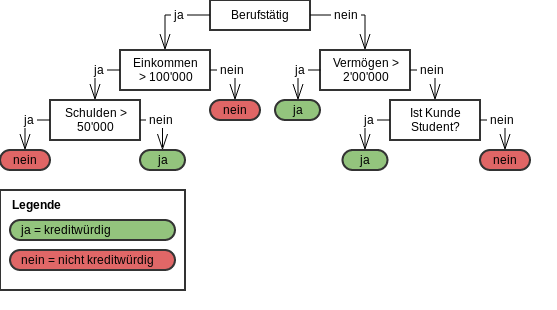
\includegraphics[width=0.8\textwidth]{images/decision_tree.png}
	\caption{Entscheidungsbaum für die Kreditwürdigkeit eines Kunden.}
	\label{fig:recherche:dataminingtechniken:disziplinen:classification}
\end{figure}

\cref{fig:recherche:dataminingtechniken:disziplinen:classification} zeigt einen Entscheidungsbaum, welcher von oben nach unten durchlaufen wird. Die Quadrate sind Entscheidungen, und bei den Ovalen handelt es sich um Zuweisungen zu der Klasse "`kreditwürdig"'.

% Evt. noch was schreiben über Training- und Testdaten

\subsubsection{Regression}
\label{sec:recherche:dataminingtechniken:disziplinen:regression}
Bei der Regresseion wird von einer abhängiger Variable Y auf eine unabhängige Grösse X zurückgeschlossen\todo{korrekt?}. Man spricht dann von einer Regression von Y auf X. Dabei werden bestehende Daten auf einem Koordinatensystem aufgetragen und eine Funktion definiert oder gesucht, welche die Messungen möglichst genau annähert. Für eine gegebene abhängige Variable kann somit die unabhängige Grösse errechnet werden\todo{cite}. 

\cref{fig:recherche:dataminingtechniken:disziplinen:regression} zeigt das Resultat einer linearen Regression.

\begin{figure}[H]
	\RawFloats
	\centering
	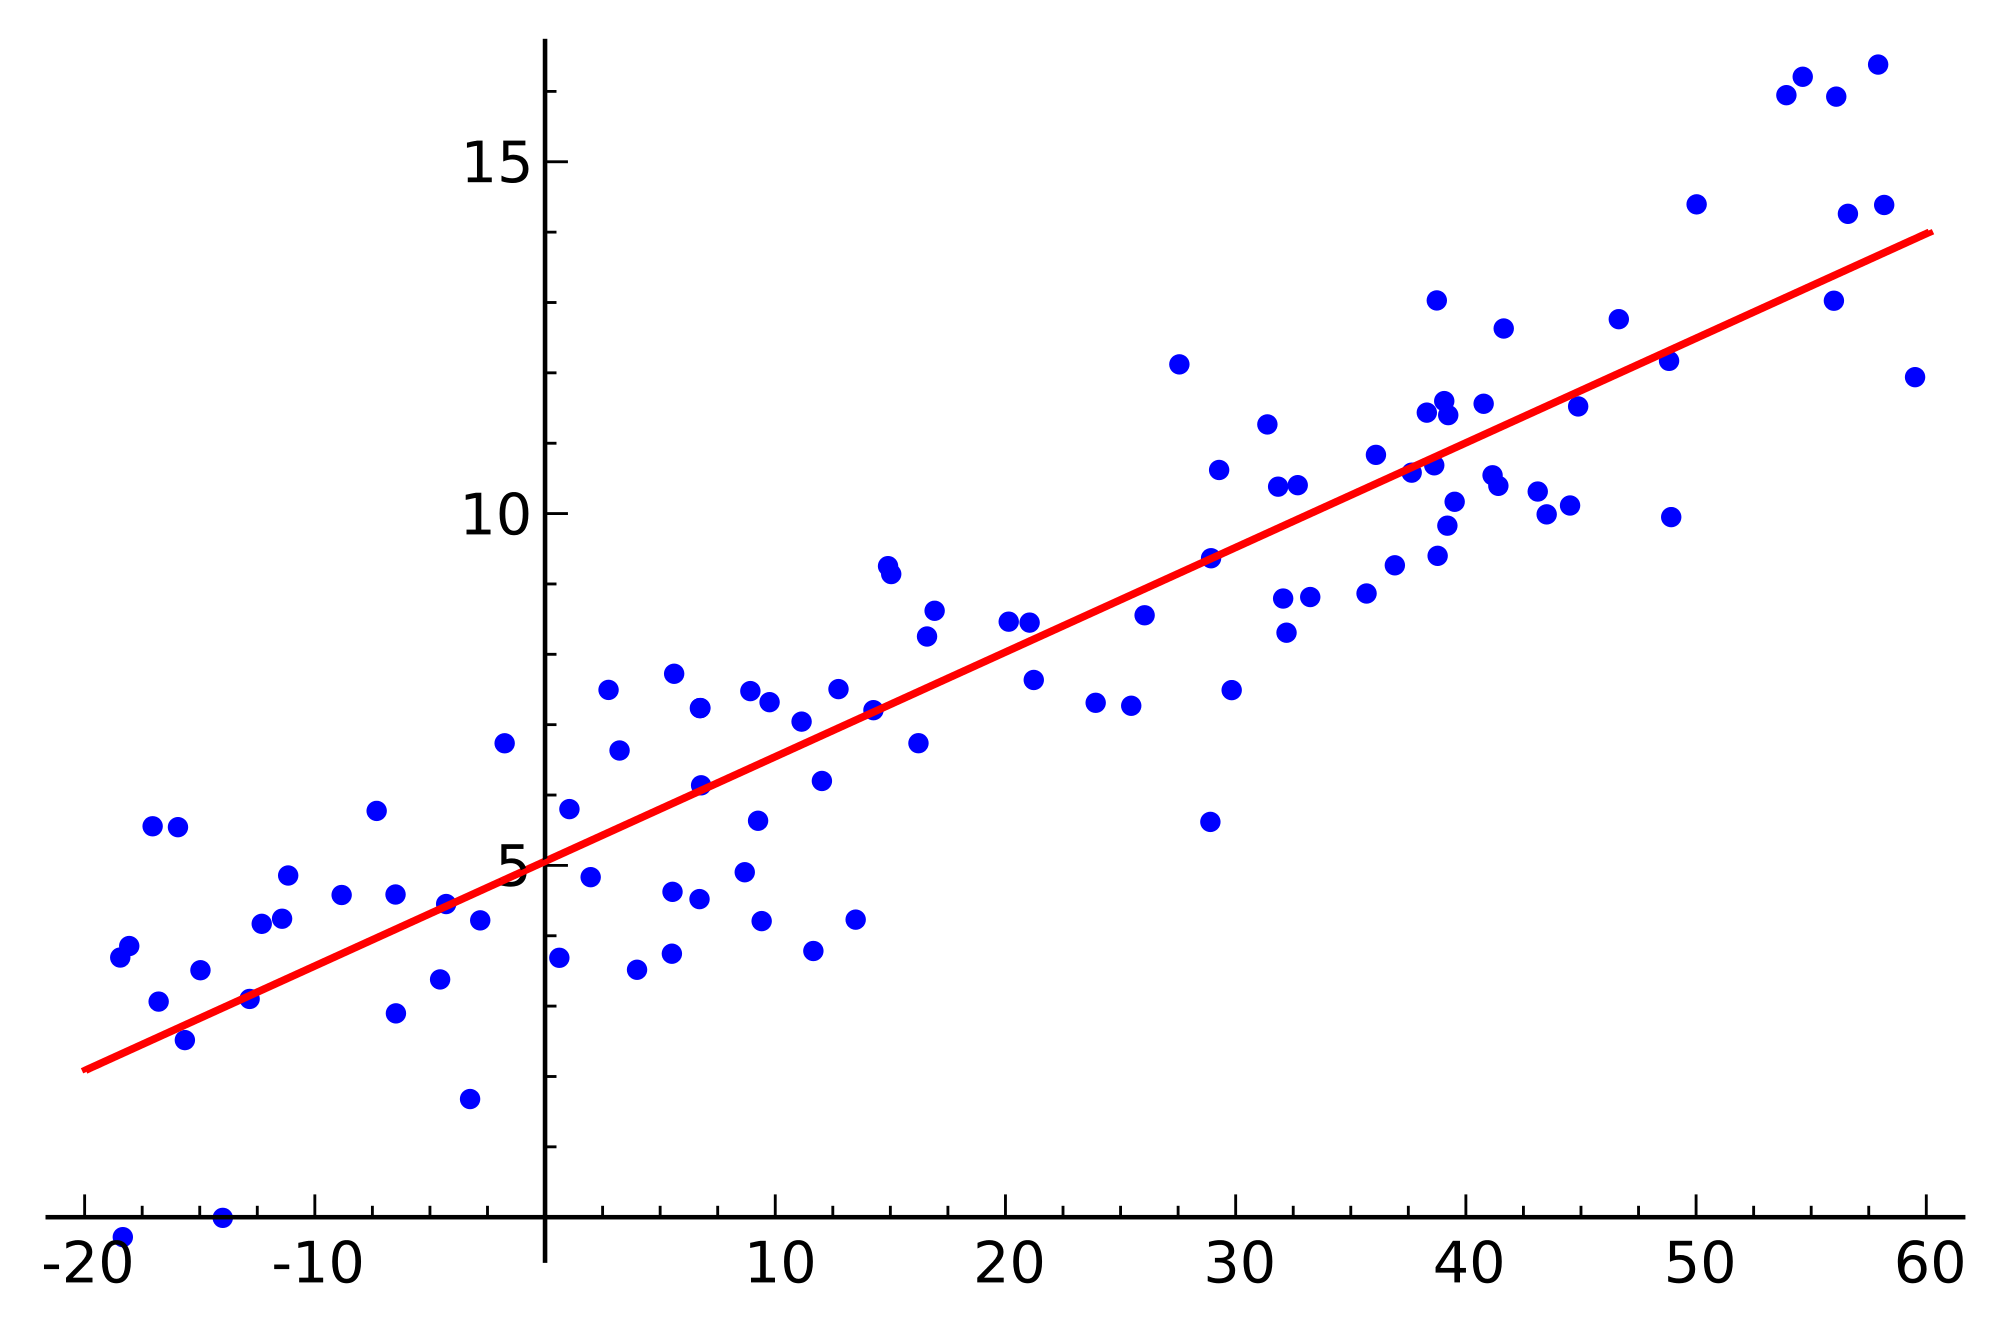
\includegraphics[width=0.8\textwidth]{images/Linear_regression.png}
	\caption{Gerade einer linearen Regression durch eine Punktwolke}
	\source{\cite{Linear_regression_2017-01-08}}
	\label{fig:recherche:dataminingtechniken:disziplinen:regression}
\end{figure}

\subsubsection{Cluster analysis}
\label{sec:recherche:dataminingtechniken:disziplinen:clusteranalysis}
Die Cluster analysis (Clusteranalyse) weist, ähnlich zur \nameref{sec:recherche:dataminingtechniken:disziplinen:classification}, den Instanzen eine Klasse zu. Jedoch sind diese zu beginn nicht bekannt, wodurch es sich um ein \gls{unsupervisedlearning} handelt.

In \cref{fig:recherche:dataminingtechniken:disziplinen:clusteranalysis} sind Punkte in einem Koordinatensystem eingetragen. Diese werden bei der Clusteranalyse in mehrere Gruppen unterteilt, welche die Klassen abbilden. Im Gegensatz zur \nameref{sec:recherche:dataminingtechniken:disziplinen:classification} haben diese jedoch keine weitere Bedeutung sondern geben nur an, dass sie ähnlich zu allen anderen Instanzen im selben Cluster sind. Je nach Verfahren ist es unterschiedlich, wie viele Klassen gebildet werden oder ob die Anzahl vorgegeben ist\footcite{data_mining_concepts_and_techniques}.
\begin{figure}[H]
	\RawFloats
	\centering
	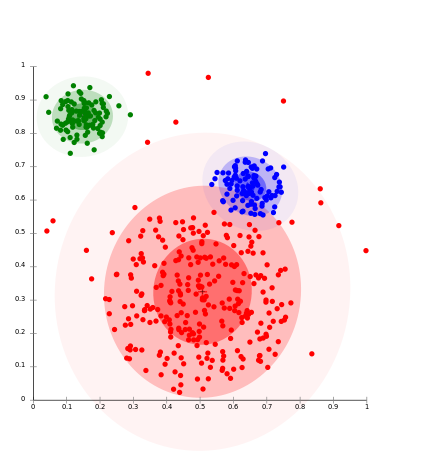
\includegraphics[width=0.8\textwidth]{images/clusteranalysis.png}
	\caption{Koordinatensystem für eine Cluster analysis}
	\source{\cite{Cluster_analysis_2017-01-08}}
	\label{fig:recherche:dataminingtechniken:disziplinen:clusteranalysis}
\end{figure}

Eingesetzt wird die Clusteranalyse zum Beispiel für die Erkennung von Kundengruppen oder zur  Zusammenfassung und Vergleich gleichartiger Produkten\footcite{einsatzgebiet_clusteranalyse}.


\subsubsection{Collaborative Filtering}
\label{sec:recherche:dataminingtechniken:disziplinen:collaborativefiltering}
Beim Collaborative Filtering (kollaboratives Filtern) wird zu einer Instanz ähnliche Objekte gesucht. Die Ähnlichkeit wird durch Bewertung von anderen Kunden errechnet. 

\begin{table}[H] 
	\caption{Begriffsdefinition}
	\centering
	\rowcolors{1}{tablebodycolor}{tablerowcolor}
	\label{fig:recherche:dataminingtechniken:disziplinen:collaborativefiltering}
	
	\begin{tabular}{ | l | c | c | c | c |} 
		\hline 
		\rowcolor{tableheadcolor}
		\bfseries & 
		\bfseries Maria & 
		\bfseries Sandro & 
		\bfseries Urs & 
		\bfseries Heidi \\ \hline 
		\textbf{Pulp Fiction} & - & - &  & + \\ \hline 
		\textbf{The Matrix} & + & + & + & - \\ \hline 
		\textbf{American Hustle} & - & + &  & + \\ \hline 
		\textbf{12 Monkeys} & + & + & - & \cellcolor{yellow!75}? \\ \hline 
	\end{tabular} 
\end{table}

Die Zeilen in der \cref{fig:recherche:dataminingtechniken:disziplinen:collaborativefiltering} sind Instanzen und die Spalten zeigen Bewertungen der Kunden. Minus steht für eine negative und Plus für eine positive Bewertung. Es ist auch möglich das ein Benutzer eine Instanz nicht bewertet. Mittels kollaborativen Filtern kann nun abgeschätzt werden, ob ein Benutzer eine Instanz positiv oder negativ Bewertet\todo{cite}.

\section{Wissenschaftliche Arbeiten}
\todo{}

\section{Programmevaluation}
\label{sec:recherche:programmevaluation}
Auf dem Markt gibt es diverse Data Mining Programme von welchen hier einige vorgestellt werden.

Zwingend notwendig ist es, dass das Programm gratis ist, sowie unter den Betriebsystemen Windows sowie Linux lauffähig ist. 

%http://thenewstack.io/six-of-the-best-open-source-data-mining-tools/

\subsection{RapidMiner Studio}
RapidMiner, früher YALE (Yet Another Learning Environment) wurde von der Technischen Universität Dortmund entwickelt und bietet eine kostenlose Version an, welche auf 10'000 Datensätze und einen logischen Prozessor beschränkt ist. Es gibt jedoch für Studenten eine Version mit welcher beliebig Grosse Daten bearbeitet werden können. Die Applikation ist in Java geschrieben und somit auf allen gängigen Betriebssystemen lauffähig\footcite{RapidMiner_Studio_2017-01-14}.

RapidMiner Studio bietet für eine grosse Anzahl an Algorithmen fertige Bausteine an, welche verwendet werden können. Alle unter \cref{sec:recherche:dataminingtechniken:disziplinen} \nameref{sec:recherche:dataminingtechniken:disziplinen} aufgeführten Methoden sind in der Applikation als Operatoren implementiert und können durch einige klicks verwendet werden. Eine Auflistung aller Operatoren ist in der RapidMiner Dokumentation aufgeführt: \url{http://docs.rapidminer.com/studio/operators/}

\subsection{Weka}
\gls{weka} ist ein in Java entwickeltes Programm der University of Waikato, New Zealand. Veröffentlicht wurde die Software unter der \gls{acr:gnugpl} und ist somit frei verfüg- und modifizierbar\footcite{Weka_2017-01-14}.

WEKA beherscht Classification, Clustering, Regression und Associating Algorithmen und deckt somit alle  im \cref{sec:recherche:dataminingtechniken:disziplinen} aufgeführten Disziplinen ab\footcite{Weka_Doc_2017-01-14}\footcite{Weka_Regression_2017-01-14}.

